%!TEX TS-program = lualatex
%!TEX encoding = UTF-8 Unicode
\documentclass[a4paper, 11pt, parskip=half]{scrartcl}

% ============================================================
% PRÄAMBEL & PAKETE (Design Herr Dayi - analog zu Freud)
% ============================================================
\usepackage[a4paper, top=1.2cm, bottom=1.2cm, left=1.8cm, right=1.6cm, footskip=0.4cm]{geometry}
\usepackage[ngerman]{babel}
\usepackage{fontspec}
\setmainfont{Libertinus Serif}
\setsansfont{Latin Modern Sans}
\usepackage{amsmath, amssymb}
\usepackage{multicol} 
\usepackage{lineno} 
\usepackage{changepage} 
\usepackage{enumitem} 
\usepackage{graphicx} 
\usepackage{qrcode}
\usepackage{xcolor}
\usepackage{colortbl}
\usepackage[most]{tcolorbox}
\usepackage{tabularx}
\usepackage{tikz}

\definecolor{primaryBlue}{RGB}{20, 50, 100} 
\definecolor{lightBlue}{RGB}{245, 248, 253}
\definecolor{accentBlue}{RGB}{37, 99, 235}

% --- Sozialform-Piktogramme ---
\newcommand{\tikzUser}[1]{%
    \begin{tikzpicture}[x=0.07cm,y=0.07cm, baseline=-0.8ex]
        \fill[#1] (0,3.5) circle (1.5);
        \fill[#1] (-2,0) .. controls (-2,1.5) and (-1.5,2) .. (0,2) .. controls (1.5,2) and (2,1.5) .. (2,0) -- (-2,0) -- cycle;
    \end{tikzpicture}%
}
\newcommand{\iconEA}{\begin{tikzpicture}[baseline=(char.base)]\node[draw=primaryBlue, thin, inner sep=2pt, fill=white] (char) {\tikzUser{primaryBlue} \scalebox{0.6}{EA}};\end{tikzpicture}}
\newcommand{\iconPA}{\begin{tikzpicture}[baseline=(char.base)]\node[draw=primaryBlue, thin, inner sep=2pt, fill=white] (char) {\tikzUser{primaryBlue}\hspace{-1pt}\tikzUser{primaryBlue} \scalebox{0.6}{PA}};\end{tikzpicture}}
\newcommand{\iconGA}{\begin{tikzpicture}[baseline=(char.base)]\node[draw=primaryBlue, thin, inner sep=2pt, fill=white] (char) {\tikzUser{primaryBlue}\hspace{-1pt}\tikzUser{primaryBlue}\hspace{-1pt}\tikzUser{primaryBlue} \scalebox{0.6}{GA}};\end{tikzpicture}}

% Aufgaben-Umgebung
\newcounter{aufgabencnt}
\newenvironment{aufgabe}[1]{ 
    \stepcounter{aufgabencnt}
    \vspace{0.18cm}
    \noindent\begin{tikzpicture}[baseline=(char.base)]
        \node[draw=primaryBlue, fill=primaryBlue, text=white, font=\small\bfseries, inner sep=2.5pt] (char) {Aufgabe \arabic{aufgabencnt}};
    \end{tikzpicture} \hspace{0.1cm} \hfill #1\par\medskip
}{%
    \par\vspace{0.1cm}
}

\newcommand{\runningMan}{%
\begin{tikzpicture}[scale=0.18, baseline=-1mm, thick]
    \draw (0,1) circle (0.4); 
    \draw (0,0.6) -- (0,-0.2); 
    \draw (0,0.4) -- (-0.6,0); 
    \draw (0,0.4) -- (0.6,0.8); 
    \draw (0,-0.2) -- (-0.5,-0.8); 
    \draw (0,-0.2) -- (0.5,0); \draw (0.5,0) -- (0.8,-0.8); 
\end{tikzpicture}}

\modulolinenumbers[5] 
\setlength\linenumbersep{9pt} 
\renewcommand\linenumberfont{\normalfont\tiny\sffamily\color{gray}}

\begin{document}

% ================= SEITE 1: TEXT UND INFOKASTEN =================

\noindent
\begin{minipage}[t]{0.30\textwidth}\textbf{Philosophie Q1} \\ Herr Dayi\end{minipage}%
\hfill
\begin{minipage}[t]{0.38\textwidth}\centering\textbf{\large Anthropologie \& Kultur (IF 3)}\end{minipage}%
\hfill
\begin{minipage}[t]{0.30\textwidth}\flushright Datum: \rule{2.5cm}{0.4pt}\end{minipage}

\vspace{0.1cm}
\hrule height 0.8pt
\vspace{0.25cm}

% --- QR-CODE MIT HILFESTELLUNG / LERNUMGEBUNG ---
\marginpar{\vspace{0.05cm}\hspace{-2.2cm}\centering%
\qrcode[height=1.2cm]{https://herrdayi.github.io/Marx/}\\[0.12cm]%
{\tiny\sffamily\color{primaryBlue}\hspace{-2.2cm}\textbf{Hilfe}}}

\noindent {\Large \textbf{\color{primaryBlue}Karl Marx – Die entfremdete Arbeit (1844)}}
\vspace{0.25cm}

% === TEXTBEREICH MIT RECHTEM NOTIZRAND (ORIGINAL MARX, GRÖSSER WIE BEI FREUD, KEINE FETTDRUCKE) ===
\begin{adjustwidth}{0cm}{1.8cm}
\normalsize\linespread{1.10}\selectfont
\begin{linenumbers}
\noindent „Das praktische Erzeugen einer gegenständlichen Welt, die Bearbeitung der unorganischen Natur ist die Bewährung des Menschen als eines bewussten Gattungswesens [\dots]. Zwar produziert auch das Tier. Es baut sich ein Nest, Wohnungen, wie die Biene, Biber, Ameise etc. Allein es produziert nur, was es unmittelbar für sich bedarf; es produziert einseitig, während der Mensch universell produziert; das Tier produziert nur unter der Herrschaft des physischen Bedürfnisses, während der Mensch frei produziert und erst wahrhaft produziert in der Freiheit [\dots] der Mensch formiert daher auch nach den Gesetzen der Schönheit.

\vspace{0.25cm}
\noindent Der Gegenstand, den die Arbeit produziert, ihr Produkt, tritt ihr als ein fremdes Wesen, als eine von dem Produzenten unabhängige Macht gegenüber. Das Produkt der Arbeit ist die Arbeit, die sich in einem Gegenstand fixiert, sachlich gemacht hat, es ist die Vergegenständlichung der Arbeit. Die Verwirklichung der Arbeit ist ihre Vergegenständlichung. Diese Verwirklichung der Arbeit erscheint in dem nationalökonomischen Zustand als Entwirklichung des Arbeiters, die Vergegenständlichung als Verlust und Knechtschaft des Gegenstandes, die Aneignung als Entfremdung, als Entäußerung. [\dots] Die Aneignung des Gegenstandes erscheint so sehr als Entfremdung, dass, je mehr Gegenstände der Arbeiter produziert, um so mehr gerät er unter die Herrschaft seines Produkts, des Kapitals. Was das Produkt seiner Arbeit ist, ist er nicht. Je größer also dies Produkt, je weniger ist er selbst.

\vspace{0.25cm}
\noindent Worin besteht nun die Entäußerung der Arbeit? Erstens, dass die Arbeit dem Arbeiter äußerlich ist, d.\,h. nicht zu seinem Wesen gehört, dass er sich daher in seiner Arbeit nicht bejaht, sondern verneint, nicht wohl, sondern unglücklich fühlt, keine freie physische und geistige Energie entwickelt, sondern seine Physis kasteit und seinen Geist ruiniert. Der Arbeiter fühlt sich daher erst außer der Arbeit und in der Arbeit außer sich. Zu Hause ist er, wenn er nicht arbeitet, und wenn er arbeitet, ist er nicht zu Hause. Seine Arbeit ist daher nicht freiwillig, sondern gezwungen, Zwangsarbeit. Sie ist nicht die Befriedigung eines Bedürfnisses, sondern nur ein Mittel, um Bedürfnisse außer ihr zu befriedigen. Ihre Fremdheit tritt dadurch rein hervor, dass, sobald kein physischer oder sonstiger Zwang existiert, die Arbeit wie eine Pest geflohen wird.

\vspace{0.25cm}
\noindent Es kommt daher zum Resultat, dass der Mensch sich nur mehr in seinen tierischen Funktionen (Essen, Trinken, Zeugen) als freitätig fühlt und in seinen menschlichen Funktionen nur mehr als Tier. Das Tierische wird das Menschliche und das Menschliche das Tierische. Essen, Trinken und Zeugen etc. sind zwar auch echt menschliche Funktionen. Aber in der Abstraktion, die sie von dem übrigen Kreis der menschlichen Betätigung trennt und zu letzten und einzigen Endzwecken macht, sind sie tierisch.“
\end{linenumbers}

\vspace{0.15cm}
\tiny {
(Originalfassung nach: Karl Marx: \textit{Ökonomisch-philosophische Manuskripte aus dem Jahre 1844}. Erstes Manuskript: \textit{Die entfremdete Arbeit}. MEW Band 40, Berlin 1968, S.~510--522.)}
\end{adjustwidth}

\vspace{0.2cm}

% === INFOKASTEN ZUR PERSON (ANALOG ZU FREUD) ===
\begin{tcolorbox}[
    enhanced, colback=lightBlue, colframe=primaryBlue, boxrule=0.8pt, arc=0mm,
    title=\textbf{Zur Person: Karl Marx (1818–1883)}, fonttitle=\small\bfseries\color{white},
    attach boxed title to top left={yshift=-2mm, xshift=2mm},
    boxed title style={colback=primaryBlue, arc=0mm, boxrule=0pt},
    boxsep=4pt, bottom=4pt, top=6pt
]
\footnotesize 
\begin{tabularx}{\textwidth}{X r}
Karl Marx war ein deutscher Philosoph, Ökonom und Gesellschaftstheoretiker. Tief geprägt von den rasanten Umbrüchen der industriellen Revolution und der wachsenden Not der Arbeiterklasse untersuchte er die materiellen Lebensbedingungen des Menschen. In seinen 1844 verfassten \textit{Ökonomisch-philosophischen Manuskripten} widmet er sich der grundlegenden Frage, welche Rolle die Arbeit für die menschliche Existenz spielt und wie die kapitalistische Produktionsweise das Verhältnis des Menschen zu sich selbst und seinen Mitmenschen prägt. & 
\raisebox{-0.85\height}{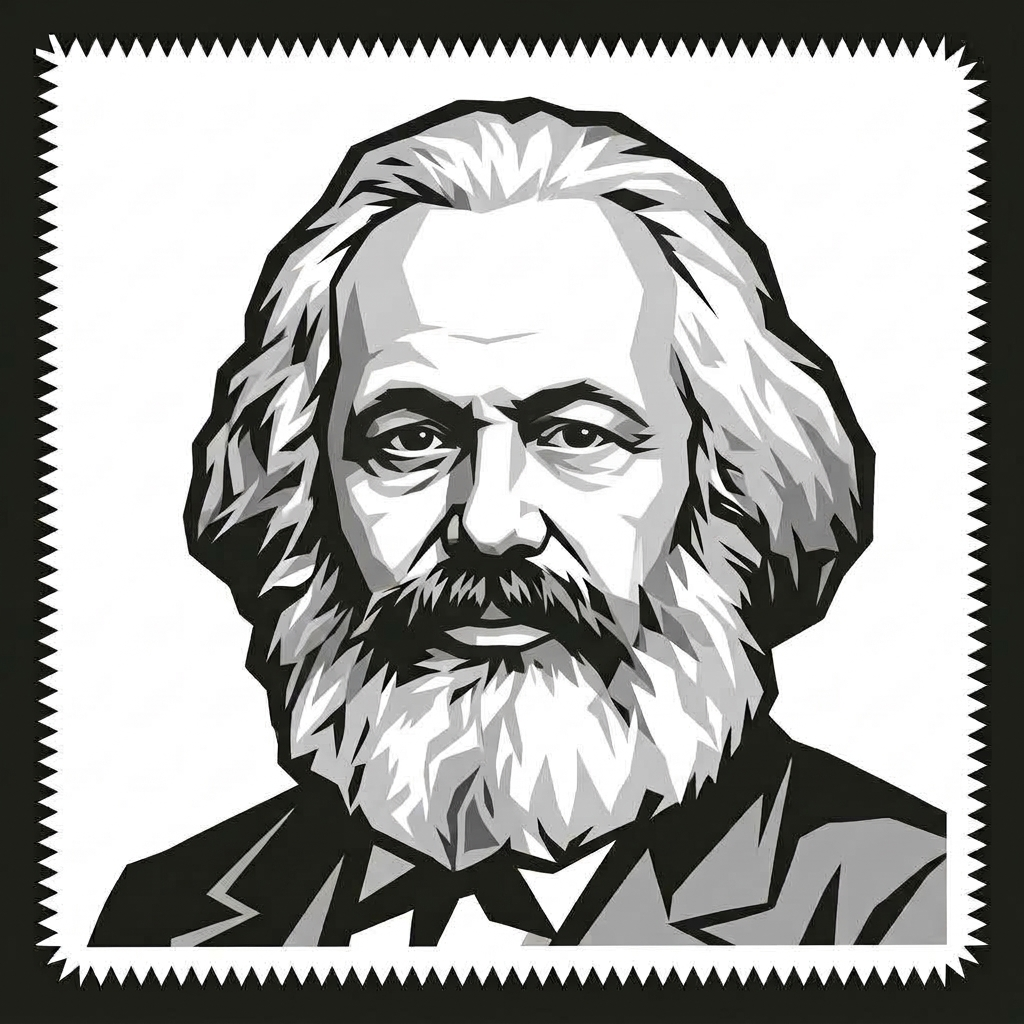
\includegraphics[width=2.1cm]{Marx.png}} 
\end{tabularx}
\end{tcolorbox}

\newpage % ================= SEITE 2: AUFGABENSTELLUNG & SICHERUNG =================

\noindent {\Large \textbf{\color{primaryBlue}Arbeitsaufträge}}
\vspace{0.15cm}

% === AUFGABE 1: THINK & GROUP ===
\begin{aufgabe}{\iconGA}
\textbf{Kernaussage erschließen:}
\begin{enumerate}[label=\alph*), leftmargin=0.5cm, itemsep=0.04cm]
    \item \textbf{Erklärt} euren zugeteilten Satzstreifen in eigenen Worten: Was will uns der Philosoph damit sagen?
    \item \textbf{Findet} ein konkretes Beispiel aus dem Alltag oder heutigen Arbeitsleben, das diesen Satz belegt oder widerlegt.
\end{enumerate}
\end{aufgabe}

% === AUFGABE 2: TEXTABGLEICH & DIMENSIONEN (OHNE FUNKTIONSPOOL) ===
\begin{aufgabe}{\iconPA \, / \, \iconGA}
\textbf{Textabgleich \& Dimensionen strukturieren:}
\begin{enumerate}[label=\alph*), leftmargin=0.5cm, itemsep=0.04cm]
    \item \textbf{Lokalisiert} euren Satz im Text (Seite~1), markiert ihn farbig und tragt die \textbf{Zeilenangabe} in die Tabelle ein.
    \item \textbf{Bestimmt} die argumentative Funktion eures Satzes sowie den Befund (Dimension der Entfremdung) und füllt die Matrix aus.
\end{enumerate}
\end{aufgabe}

\vspace{0.1cm}

% === MATRIX TABELLE (MIT ZEILENANGABEN STATT SEITEN) ===
\begin{tcolorbox}[
    enhanced, colback=white, colframe=primaryBlue, boxrule=0.8pt, arc=0mm,
    title=\textbf{Tafelsicherung: Die 4 Dimensionen der Entfremdung bei Karl Marx},
    fonttitle=\small\bfseries\color{white},
    attach boxed title to top left={yshift=-2mm, xshift=2mm},
    boxed title style={colback=primaryBlue, arc=0mm, boxrule=0pt},
    boxsep=3pt, bottom=3pt, top=5pt
]
\footnotesize\sffamily
\renewcommand{\arraystretch}{1.12}
\begin{tabularx}{\textwidth}{|p{3.2cm}|p{3.8cm}|X|}
\hline
\rowcolor{lightBlue}
\textbf{\color{primaryBlue}Kernaussage} & 
\textbf{\color{primaryBlue}Argumentative Funktion} & 
\textbf{\color{primaryBlue}Entfremdungsdimension / Befund} \\
\hline
\textbf{Satz A} \newline {\scriptsize Zeile: \rule{1.4cm}{0.4pt}} \newline \scriptsize (Gattungswesen) & \rule{0pt}{0.85cm} & \\
\hline
\textbf{Satz B} \newline {\scriptsize Zeile: \rule{1.4cm}{0.4pt}} \newline \scriptsize (Herrschaft d. Produkts) & \rule{0pt}{0.85cm} & \\
\hline
\textbf{Satz C} \newline {\scriptsize Zeile: \rule{1.4cm}{0.4pt}} \newline \scriptsize (Zwangsarbeit) & \rule{0pt}{0.85cm} & \\
\hline
\textbf{Satz D} \newline {\scriptsize Zeile: \rule{1.4cm}{0.4pt}} \newline \scriptsize (Paradoxon) & \rule{0pt}{0.85cm} & \\
\hline
\end{tabularx}
\end{tcolorbox}

\vspace{0.1cm}

% === AUFGABE 3: TRANSFER & KULTUR-URTEIL ===
\begin{aufgabe}{\iconPA \, $\rightarrow$ \, \iconEA}
\textbf{Kultur-Urteil fällen:}
\begin{enumerate}[label=\alph*), leftmargin=0.5cm, itemsep=0.04cm]
    \item \textbf{Vergleicht:} Gehlen sieht Kultur als Entlastung, Freud als seelische Belastung (Triebverzicht). Was sagt Marx anhand der 4 Sätze über die Kultur unserer Arbeitswelt?
    \item \textbf{Blitz-Urteil zu Satz D:} Stimmt das heute noch? Fühlen wir uns nach Schule/Arbeit wirklich nur noch beim Essen, Trinken und Binge-Watching als freier Mensch -- und in der Arbeit wie dressierte Tiere?
\end{enumerate}
\end{aufgabe}

\vspace{0.2cm}

% === METHODISCHER BAUSTEIN AM ENDE DER SEITE 2 (OHNE FETTDRUCKE AM ANFANG, OHNE STAMMBEREICHE) ===
\begin{tcolorbox}[
    enhanced, colback=lightBlue, colframe=primaryBlue, boxrule=0.8pt, arc=1mm,
    title=\textbf{Methode: Kernaussagen-Rekonstruktion},
    fonttitle=\small\bfseries\color{white},
    boxed title style={colback=primaryBlue, arc=0mm, boxrule=0pt},
    attach boxed title to top left={yshift=-2mm, xshift=2mm},
    boxsep=4pt, bottom=5pt, top=6pt
]
\small\sffamily
\begin{enumerate}[leftmargin=0.55cm, itemsep=0.08cm, topsep=0.04cm]
    \item Erschließt eure isolierte Kernstelle in der Kleingruppe, formuliert die Aussage in eigenen Worten und findet ein passendes Alltagsbeispiel.
    \item Ordnet die Thesen gemeinsam im Kurs in eine logische Abfolge (Ursache $\rightarrow$ Folge) und begründet eure Kurshypothese.
    \item Überprüft die Vermutung anhand des Originaltextes und bestimmt die argumentative Funktion sowie die Dimension der Entfremdung.
\end{enumerate}
\end{tcolorbox}

\end{document}
